\chapter{Vervolg}
\label{ch:vervolg}

In dit hoofdstuk zullen mogelijke vervolgen en toepassingen van deze bachelorproef beschreven worden. Hoe kunnen anderen toegang krijgen tot de programmeercode, de website raadplegen of hoe kan de \textit{webserver} geïnstalleerd worden binnen het HOGENT-netwerk. Ook zal er besproken worden hoe de data beter en objectiever gelabeld kan worden. Omdat het doelpubliek van dit hoofdstuk anders dan het doelpubliek van het meer technische luik van dit onderzoek, zal alles zo makkelijk mogelijk uitgelegd worden.

\section{Applicatie-code delen}
Om er zeker van te zijn dat deze bachelorproef niet onder het stof verdwijnt en dat de applicatie niet meer gebruikt zal worden, is het noodzakelijk dat de volledige programmacode gedeeld kan worden. Hiervoor zal er gebruik gemaakt worden van ``GitHub''.

Om GitHub te begrijpen is het eerst nodig te begrijpen wat Git zelf is. Git is een open source versiebeheersysteem. Telkens ontwikkelaars met de eigen code aan de slag gaan en hun eigen wijzigingen aanbrengen, worden op die manier de verschillen in code opgeslagen. Versiebeheersystemen beheren deze revisies door alle wijzigingen op te slaan in een centrale opslagplaats. Hierdoor kunnen ontwikkelaars gemakkelijk samenwerken, omdat ze een nieuwe versie van de software kunnen downloaden, wijzigen en zelf nieuwe revisies kunnen uploaden. Elke programmeur van dat project kan dan op zijn of haar beurt opnieuw zien welke wijzigingen er doorgevoerd zijn en kan deze opnieuw downloaden.~\autocite{Brown2019}

GitHub is dus zo een voorbeeld van een centrale opslagplaats waar alle wijzigingen opgeslagen staan in de \textit{cloud}.

Alle code, bestanden en revisies van deze volledige bachelorproef zijn dan ook te vinden op de persoonlijke GitHub-link: \url{https://github.com/SibianDG/BachelorProef}. Wanneer iemand toegang wil, dan kan men een e-mail sturen naar Jorrit Campens die u dan in contact brengt met de schrijver, Sibian De Gussem.

\section{Hosting en bereikbaarheid van de applicatie}
Om te kunnen spreken hoe we het beste de applicatie beschikbaar maken, is het eerst noodzakelijk dat iedereen weet wat dat allemaal betekent.

De huidige opstelling van dit eindwerk is geïllustreerd in figuur~\ref{fig:opstelling_bachelorproef}. Daarbij is alle code geïnstalleerd, of eerder gezegd aanwezig op die lokale computer zelf. Wanneer het bestand `website.py' wordt uitgevoerd, zal Python de code uitvoeren en een webserver opzetten op die lokale machine. In de output verschijnt er dan een website-adres. Als er naar de website gegaan wordt ziet u de applicatie.

\begin{figure}
    \centering
    
\includegraphics[width=0.75\textwidth]{./img/lokaal_website}
    \caption{\label{fig:opstelling_bachelorproef} Opstelling bachelorproef}
\end{figure}

Wanneer we de website beschikbaar willen maken voor meerdere computers moeten we de code op een server installeren, maar een server kan ook een gewone computer zijn. Zo kunnen er meerde \textit{clients} een aanvraag of \textit{request} sturen naar de server die alles afhandelt zoals de webpagina tonen en de berekeningen uitvoeren. Een illustratie is te vinden op figuur~\ref{fig:webhosting_scheme}. Daarbij is te zien dat wanneer een gebruiker of \textit{user} naar een website surft, er een verzoek verstuurd wordt naar het internet. Het internet weet op zijn beurt aan welke webserver die informatie kan vragen of sturen. De server handelt de website zelf af, de html-, en JavaScript-pagina's als websitebestanden, en doet ook de berekeningen.

\begin{figure}
    \centering
    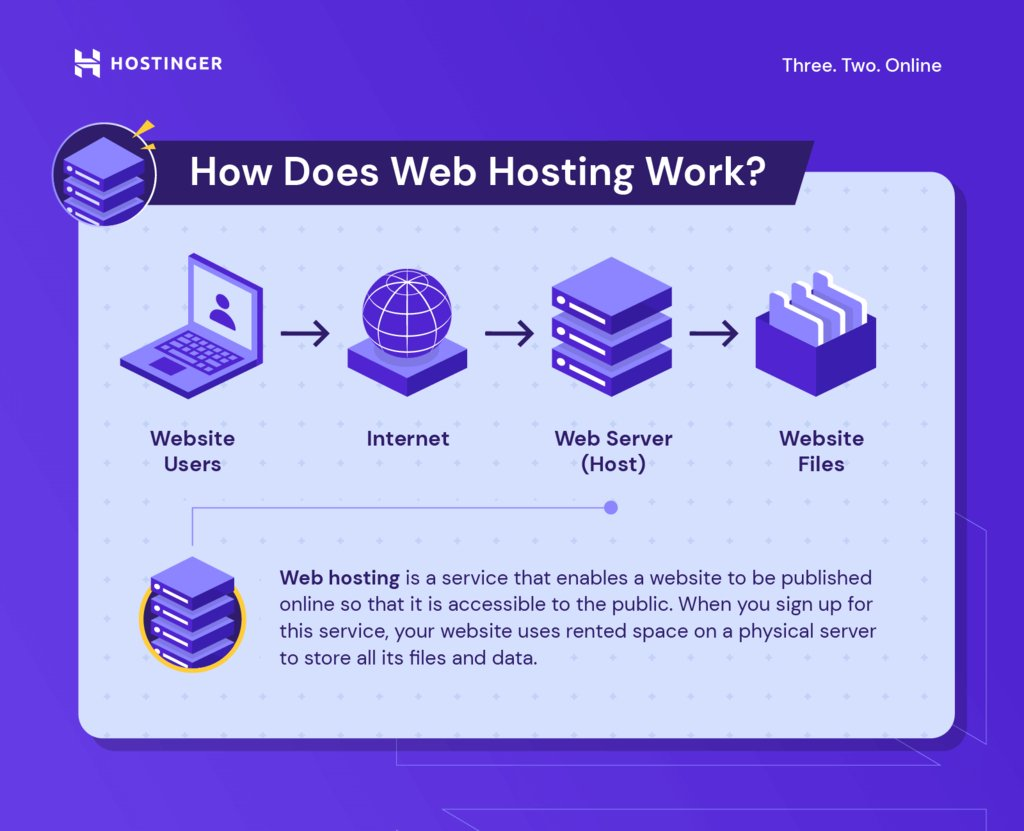
\includegraphics[width=0.8\textwidth]{./img/how-does-web-hosting-work}
    \caption{\label{fig:webhosting_scheme} Hoe werkt webhosting.~\autocite{Tamara2022}}
\end{figure}

\subsection{Installeren op een computer}
Hoe kan men alles installeren op een enkele computer?
In de hoofdmap met alle code is er een bestand te vinden genaamd ``requirements.txt''. Door het commando:
\begin{python}
    pip install -r requirements.txt
\end{python}
uit te voeren zullen alle Python-bibliotheken geïnstalleerd worden die nodig zijn om het project uit te voeren. Op Windows moet er wel nog een extra stap gebeuren en dat is FFmpeg apart installeren. De stappen daarvan staan beschreven op de volgende website: \url{https://www.wikihow.com/Install-FFmpeg-on-Windows}.

\subsubsection{Mogelijkheden}
\begin{itemize}
    \item Snelle opzet voor IT'ers
    \item Snelle verwerking omdat het op dezelfde computer gebeurt en er maar een persoon aan kan
    \item Gratis oplossing
\end{itemize}
\subsubsection{Beperkingen}
\begin{itemize}
    \item Andere computers hebben geen toegang
    \item Niet-IT'ers kunnen het mogelijk minder makkelijk installeren
    \item Alles zou geïnstalleerd moeten worden op elke computer opnieuw
\end{itemize}

\subsection{Hosten in een lokaal netwerk}
Het is ook mogelijk om de software op een computer te installeren, deze te laten aanstaan, maar met een speciale parameter. Wanneer er in de Flask-applicatie de volgende parameter wordt meegegeven: `` host=`0.0.0.0' '', zal de applicatie opengesteld worden in het lokale netwerk. Dit laat het mogelijk naar het lokale IP-adres de surfen op een ander toestel en ook de website met de detector te kunnen gebruiken. Als men het argument \textit{threaded} op \textit{true} zet, dan is Flask \textit{multithreaded}~\autocite{Vieira2013}. Hierdoor kunnen er zeker meerdere verbindingen tegelijk verbonden worden. Een systematische voorstelling is te vinden in figuur~\ref{fig:lokaal_netwerk}

\subsubsection{Mogelijkheden}
\begin{itemize}
    \item Een keer installeren op een computer van bijvoorbeeld de docent in kwestie, en nadien kan het programma altijd opgestart worden tijdens een les.
    \item Meerdere connecties mogelijk
    \item Een gratis oplossing
\end{itemize}
\subsubsection{Beperkingen}
\begin{itemize}
    \item Het maximale aantal connecties is afhankelijk van de computer waar de applicatie wordt opgestart. Hoe beter en sneller de computer, hoe meer connecties mogelijk en hoe sneller.
\end{itemize}

\begin{figure}
    \centering
    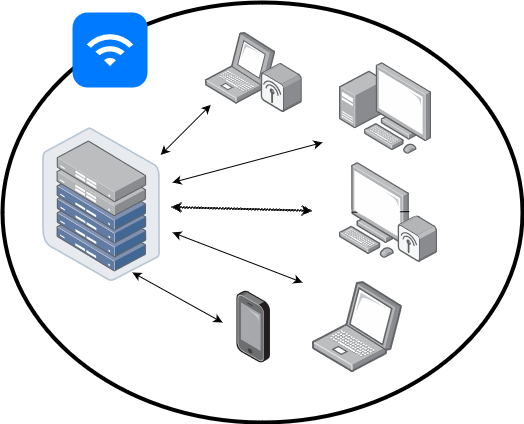
\includegraphics[width=0.75\textwidth]{./img/lokaal_netwerk}
    \caption{\label{fig:lokaal_netwerk} Lokaal netwerk}
\end{figure}

\subsection{Gratis hosting online}
De applicatie kan ook online gehost worden, maar dit zal natuurlijk geld kosten. Zo'n applicatie kan dan gehost worden op Microsoft Azure als webapplicatie.
\subsubsection{Mogelijkheden}
\begin{itemize}
    \item Eens opgezet is het altijd beschikbaar van overal
    \item Wanneer er veel verbindingen en berekeningen nodig zijn, zal Microsoft de servers \textit{upgraden} zodat ze alles kunnen bolwerken
    \item Heel snel
\end{itemize}
\subsubsection{Beperkingen}
\begin{itemize}
    \item Kost veel geld
\end{itemize}
\section{Testen}
De testen die verzameld zijn, is niet van een bijzonder grote grootteorde. Er kunnen extra testen in de vorm van nieuwe audio-opnames opgenomen worden in een vervolgopdracht. Dit kan een interdisciplinaire opdracht zijn met de richting verpleegkunde en/of communicatie en eventueel samen met de richting toegepaste informatica. Hoe meer testen, hoe accurater de productiviteit van de applicatie.

Een opdracht bij de richting verpleegkunde kan het volgende zijn: de studenten maken en/of klasseren audio-opnames van eventuele \textit{elderspeak}. Hierna kan de gelabelde data gevoed worden aan het Python-script dat er geschreven is voor deze bachelorproef. Hierna kan er achterhaald worden hoe goed de applicatie presteert.

In een richting van communicatie kan alle data opnieuw gelabeld worden, waar men veel kennis heeft rond dit fenomeen. Zo kan de data zeer nauwkeurig en uitgebreid geanalyseerd worden, terwijl er in dit eindwerk de data gelabeld is door een persoon die geen expert is.

Ook kan dit een opdracht vormen voor studenten toegepaste informatica om de gelabelde data naar de server door te sturen en een resultaat terug te krijgen. Dit is wel al beschikbaar in deze bachelorproef, maar studenten die dat nog moeten leren kunnen zo een echt voorbeeld hebben iets te programmeren. Wanneer de data uitgebreider geanalyseerd wordt, moeten de testen lichtjes herschreven worden, dus dit kan ook een voorbeeld zijn van een opdracht.
